\input{bmsLayoutPage}

\usetikzlibrary{angles, quotes, calc, babel}


\renewcommand{\bbwAufgabenBlockID}{AllgDreieck}

\renewcommand{\metaHeaderLine}{Allgemeines Dreieck}
\renewcommand{\arbeitsblattTitel}{Sinus- und Cosinussatz}

\ifisNURAUFGABEN
\renewcommand{\abplz}[1]{\vspace{1mm}}
\fi

\newcommand{\seitenUmbruchImAufgabenteil}{
\ifisNURAUFGABEN
\else
\noTRAINER{\newpage}
\fi
}%%

\begin{document}
\arbeitsblattHeader{}

\begin{center}V 0.1 (2026-02-03) \end{center}
\section{Teil 1; Aufgaben mit Skizzen}


\textit{Berechnen Sie die gesuchten Größen (markiert mit ?). Die Skizzen sind nicht maßstabsgetreu.}

\subsection*{A) Sinussatz: Seite berechnen}
\begin{minipage}[t]{0.48\textwidth}
    \begin{enumerate}[series=aufgaben]
        \item $b = ?$\\
        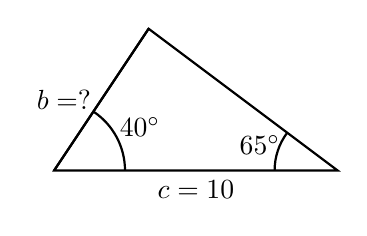
\begin{tikzpicture}[scale=1.2, thick]
            \coordinate (A) at (0,0); \coordinate (B) at (3,0); \coordinate (C) at (1,1.5);
            \draw (A) -- (B) node[midway, below]{$c=10$} -- (C) -- cycle;
            \draw (A) -- (C) node[midway, left]{$b=?$};
            \pic[draw, angle radius=0.9cm, "\,\,$40^\circ$", angle eccentricity=1.3] {angle = B--A--C};
            \pic[draw, angle radius=0.8cm, "$65^\circ$", angle eccentricity=1.3] {angle = C--B--A};
        \end{tikzpicture}
    \end{enumerate}
\end{minipage}
\hfill
\begin{minipage}[t]{0.48\textwidth}
    \begin{enumerate}[resume=aufgaben]
        \item $a = ?$\\
        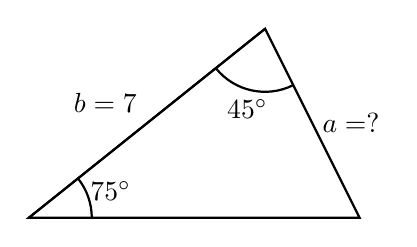
\begin{tikzpicture}[scale=1.2, thick]
            \coordinate (A) at (0,0); \coordinate (B) at (3.5,0); \coordinate (C) at (2.5,2);
            \draw (A) -- (B) -- (C) node[midway, right]{$a=?$} -- cycle;
            \draw (A) -- (C) node[midway, above left]{$b=7$};
            \pic[draw, angle radius=0.8cm, "\,\,$75^\circ$", angle eccentricity=1.3] {angle = B--A--C};
            \pic[draw, angle radius=0.8cm, "$45^\circ$", angle eccentricity=1.3] {angle = A--C--B};
        \end{tikzpicture}
    \end{enumerate}
\end{minipage}

\TNTeop{}


\subsection*{B) Sinussatz: Winkel berechnen}
\begin{minipage}[t]{0.48\textwidth}
    \begin{enumerate}[resume=aufgaben]
        \item $\beta = ?$\\
        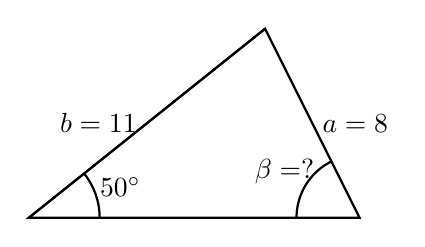
\begin{tikzpicture}[scale=1.2, thick]
            \coordinate (A) at (0,0); \coordinate (B) at (3.5,0); \coordinate (C) at (2.5,2);
            \draw (A) -- (B) -- (C) node[midway, right]{$a=8$} -- cycle;
            \draw (A) -- (C) node[midway, left]{$b=11$};
            \pic[draw, angle radius=0.9cm, "\,\,$50^\circ$", angle eccentricity=1.3] {angle = B--A--C};
            \pic[draw, angle radius=0.8cm, "$\beta=?$", angle eccentricity=1.4] {angle = C--B--A};
        \end{tikzpicture}
    \end{enumerate}
\end{minipage}

\TNTeop{}





\subsection*{C) Sinussatz: Stumpfwinklige Dreiecke}
\begin{minipage}[t]{0.48\textwidth}
    \begin{enumerate}[resume=aufgaben]
        \item $\gamma = ?$ \\
        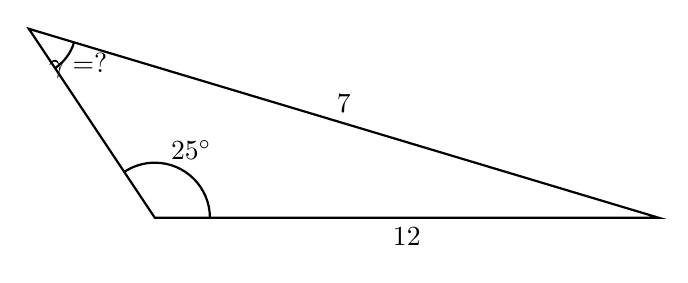
\begin{tikzpicture}[scale=1.6, thick]
            \coordinate (A) at (0,0); \coordinate (B) at (4,0); \coordinate (C) at (-1,1.5);
            \draw (A) -- (B) node[midway, below]{$12$} -- (C) node[midway, above]{$7$} -- cycle;
            \pic[draw, angle radius=0.7cm, "$25^\circ$", angle eccentricity=1.4] {angle = B--A--C};
            \pic[draw, angle radius=0.6cm, "$\gamma=?$", angle eccentricity=1.3] {angle = A--C--B};
        \end{tikzpicture}
    \end{enumerate}
\end{minipage}
\hfill
\begin{minipage}[t]{0.48\textwidth}
    \begin{enumerate}[resume=aufgaben]
        \item $\alpha = ?$ \\
        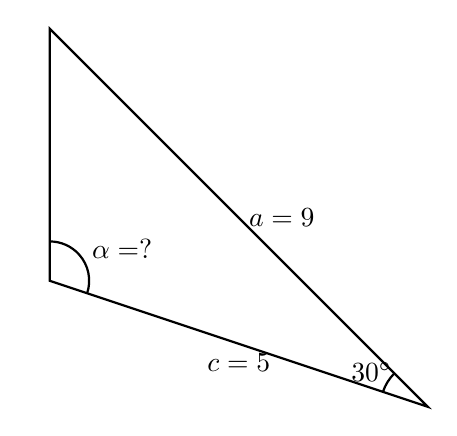
\begin{tikzpicture}[scale=1.6, thick]
            \coordinate (A) at (0,0); \coordinate (B) at (3,-1); \coordinate (C) at (0,2);
            \draw (A) -- (B) node[midway, below]{$c=5$} -- (C) node[midway, right]{$a=9$} -- cycle;
            \pic[draw, angle radius=0.5cm, "\hspace{7mm}$\alpha=?$", angle eccentricity=1.4] {angle = B--A--C};
            \pic[draw, angle radius=0.6cm, "$30^\circ$", angle eccentricity=1.4] {angle = C--B--A};
        \end{tikzpicture}
    \end{enumerate}
\end{minipage}

\vspace{0.5cm}

\begin{minipage}[t]{0.48\textwidth}
    \begin{enumerate}[resume=aufgaben]
        \item $\beta = ?$ \\
        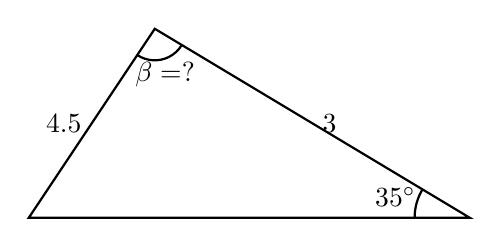
\begin{tikzpicture}[scale=1.6, thick]
            \coordinate (A) at (0,0); \coordinate (B) at (1,1.5); \coordinate (C) at (3.5,0);
            \draw (A) -- (B) node[midway, left]{$4.5$} -- (C) node[midway, right]{$3$} -- cycle;
            \pic[draw, angle radius=0.4cm, "$\beta=?$", angle eccentricity=1.5] {angle = A--B--C};
            \pic[draw, angle radius=0.7cm, "$35^\circ$", angle eccentricity=1.4] {angle = B--C--A};
        \end{tikzpicture}
    \end{enumerate}
\end{minipage}


\TNTeop{}



\subsection*{D) Cosinussatz: Seite berechnen}
\begin{minipage}[t]{0.48\textwidth}
    \begin{enumerate}[resume=aufgaben]
        \item $c = ?$\\
        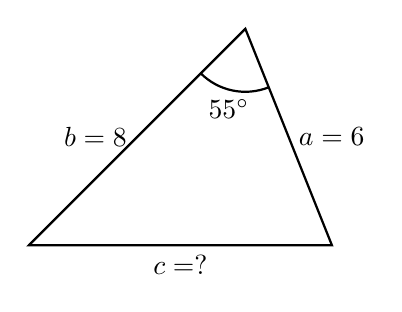
\begin{tikzpicture}[scale=1.1, thick]
            \coordinate (A) at (0,0); \coordinate (B) at (3.5,0); \coordinate (C) at (2.5,2.5);
            \draw (A) -- (B) node[midway, below]{$c=?$} -- (C) node[midway, right]{$a=6$} -- cycle;
            \draw (A) -- (C) node[midway, left]{$b=8$};
            \pic[draw, angle radius=0.8cm, "$55^\circ$", angle eccentricity=1.3] {angle = A--C--B};
        \end{tikzpicture}
    \end{enumerate}
\end{minipage}
\hfill
\begin{minipage}[t]{0.48\textwidth}
    \begin{enumerate}[resume=aufgaben]
        \item $b = ?$\\
        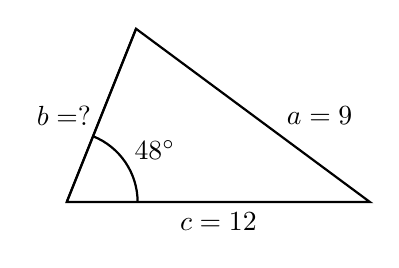
\begin{tikzpicture}[scale=1.1, thick]
            \coordinate (A) at (0,0); \coordinate (B) at (3.5,0); \coordinate (C) at (0.8,2);
            \draw (A) -- (B) node[midway, below]{$c=12$} -- (C) node[midway, right]{\hspace{3mm}$a=9$} -- cycle;
            \draw (A) -- (C) node[midway, left]{$b=?$};
            \pic[draw, angle radius=0.9cm, "\hspace{3mm}$48^\circ$", angle eccentricity=1.3] {angle = B--A--C};
        \end{tikzpicture}
    \end{enumerate}
\end{minipage}

\TNTeop{}





\subsection*{E) Cosinussatz: Winkel berechnen}
\begin{minipage}[t]{0.48\textwidth}
    \begin{enumerate}[resume=aufgaben]
        \item $\alpha = ?$\\
        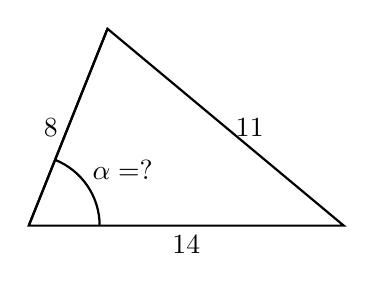
\begin{tikzpicture}[scale=1.0, thick]
            \coordinate (A) at (0,0); \coordinate (B) at (4,0); \coordinate (C) at (1,2.5);
            \draw (A) -- (B) node[midway, below]{$14$} -- (C) node[midway, right]{$11$} -- cycle;
            \draw (A) -- (C) node[midway, left]{$8$};
            \pic[draw, angle radius=0.9cm, "\hspace{3mm}$\alpha=?$", angle eccentricity=1.4] {angle = B--A--C};
        \end{tikzpicture}
    \end{enumerate}
\end{minipage}
\hfill
\begin{minipage}[t]{0.48\textwidth}
    \begin{enumerate}[resume=aufgaben]
        \item $\gamma = ?$\\
        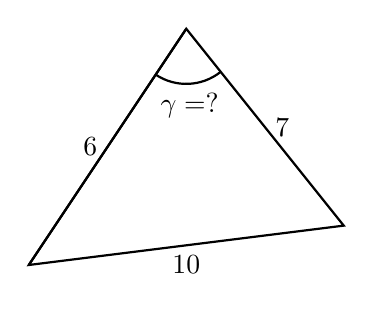
\begin{tikzpicture}[scale=1.0, thick]
            \coordinate (A) at (0,0); \coordinate (B) at (4,0.5); \coordinate (C) at (2,3);
            \draw (A) -- (B) node[midway, below]{$10$} -- (C) node[midway, right]{$7$} -- cycle;
            \draw (A) -- (C) node[midway, left]{$6$};
            \pic[draw, angle radius=0.7cm, "$\gamma=?$", angle eccentricity=1.4] {angle = A--C--B};
        \end{tikzpicture}
    \end{enumerate}
\end{minipage}

\TNTeop{}



\subsection*{F) Vermischte Aufgaben mit Skizzen}
\begin{minipage}[t]{0.32\textwidth}
    \begin{enumerate}[resume=aufgaben]
        \item $x = ?$ \\
        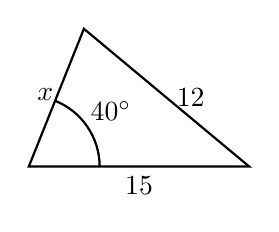
\begin{tikzpicture}[scale=0.7, thick]
            \coordinate (A) at (0,0); \coordinate (B) at (4,0); \coordinate (C) at (1,2.5);
            \draw (A) -- (B) node[midway, below]{$15$} -- (C) node[midway, right]{$12$} -- cycle;
            \pic[draw, angle radius=0.9cm, "$40^\circ$", angle eccentricity=1.4] {angle = B--A--C};
            \node at (0.3, 1.3) {$x$};
        \end{tikzpicture}
    \end{enumerate}
\end{minipage}
\hfill
\begin{minipage}[t]{0.32\textwidth}
    \begin{enumerate}[resume=aufgaben]
        \item $\beta = ?$ \\
        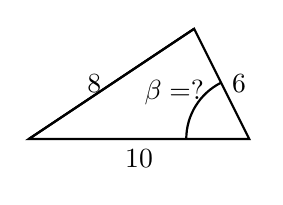
\begin{tikzpicture}[scale=0.7, thick]
            \coordinate (A) at (0,0); \coordinate (B) at (4,0); \coordinate (C) at (3,2);
            \draw (A) -- (B) node[midway, below]{$10$} -- (C) node[midway, right]{$6$} -- cycle;
            \draw (A) -- (C) node[midway, left]{$8$};
            \pic[draw, angle radius=0.8cm, "$\beta=?$", angle eccentricity=1.4] {angle = C--B--A};
        \end{tikzpicture}
    \end{enumerate}
\end{minipage}
\hfill
\begin{minipage}[t]{0.32\textwidth}
    \begin{enumerate}[resume=aufgaben]
        \item $y = ?$ \\
        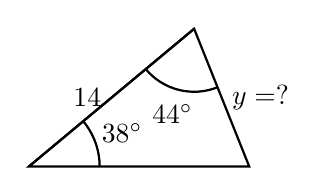
\begin{tikzpicture}[scale=0.7, thick]
            \coordinate (A) at (0,0); \coordinate (B) at (4,0); \coordinate (C) at (3,2.5);
            \draw (A) -- (B) -- (C) node[midway, right]{$y=?$} -- cycle;
            \draw (A) -- (C) node[midway, left]{$14$};
            \pic[draw, angle radius=0.9cm, "$38^\circ$", angle eccentricity=1.4] {angle = B--A--C};
            \pic[draw, angle radius=0.8cm, "$44^\circ$", angle eccentricity=1.4] {angle = A--C--B};
        \end{tikzpicture}
    \end{enumerate}
\end{minipage}

\vspace{0.8cm}

\begin{minipage}[t]{0.32\textwidth}
    \begin{enumerate}[resume=aufgaben]
        \item $\alpha = ?$ \\
        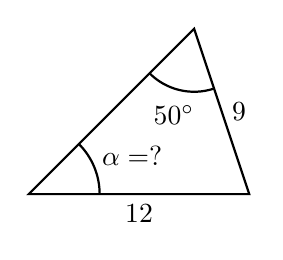
\begin{tikzpicture}[scale=0.7, thick]
            \coordinate (A) at (0,0); \coordinate (B) at (4,0); \coordinate (C) at (3,3);
            \draw (A) -- (B) node[midway, below]{$12$} -- (C) node[midway, right]{$9$} -- cycle;
            \pic[draw, angle radius=0.9cm, "\hspace{3mm}$\alpha=?$", angle eccentricity=1.4] {angle = B--A--C};
            \pic[draw, angle radius=0.8cm, "$50^\circ$", angle eccentricity=1.4] {angle = A--C--B};
        \end{tikzpicture}
    \end{enumerate}
\end{minipage}
\hfill
\begin{minipage}[t]{0.32\textwidth}
    \begin{enumerate}[resume=aufgaben]
        \item $z = ?$ \\
        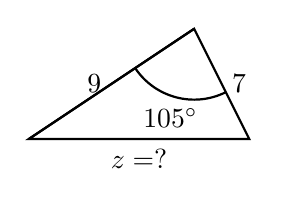
\begin{tikzpicture}[scale=0.7, thick]
            \coordinate (A) at (0,0); \coordinate (B) at (4,0); \coordinate (C) at (3,2);
            \draw (A) -- (B) node[midway, below]{$z=?$} -- (C) node[midway, right]{$7$} -- cycle;
            \draw (A) -- (C) node[midway, left]{$9$};
            \pic[draw, angle radius=0.9cm, "$105^\circ$", angle eccentricity=1.3] {angle = A--C--B};
        \end{tikzpicture}
    \end{enumerate}
\end{minipage}
\hfill
\begin{minipage}[t]{0.32\textwidth}
    \begin{enumerate}[resume=aufgaben]
        \item $\epsilon = ?$ \\
        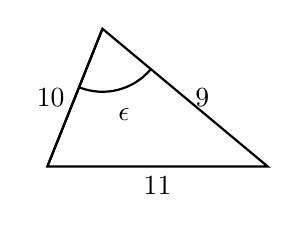
\begin{tikzpicture}[scale=0.7, thick]
            \coordinate (A) at (0,0); \coordinate (B) at (4,0); \coordinate (C) at (1,2.5);
            \draw (A) -- (B) node[midway, below]{$11$} -- (C) node[midway, right]{$9$} -- cycle;
            \draw (A) -- (C) node[midway, left]{$10$};
            \pic[draw, angle radius=0.8cm, "$\epsilon$", angle eccentricity=1.4] {angle = A--C--B};
        \end{tikzpicture}
    \end{enumerate}
\end{minipage}

\vspace{1cm}

\TNTeop{}



\section*{Teil 2: Vermischte Aufgaben in Textform}
\textit{Skizzieren Sie das Dreieck $ABC$ zuerst selbstständig.}

\begin{enumerate}[resume=aufgaben]
    \item Gegeben sind $a = 5,4$ cm, $b = 7,2$ cm und $c = 9,0$ cm. Berechnen Sie den Winkel $\beta$.
    \item Im Dreieck $ABC$ sind $b = 12$ m, $\beta = 45^\circ$ und $\gamma = 70^\circ$. Berechnen Sie die Länge der Seite $c$.
    \item Gegeben sind $a = 8,5$ cm, $c = 6,2$ cm und der eingeschlossene Winkel $\beta = 115^\circ$. Berechnen Sie die Seite $b$.
    \item Im Dreieck sind $b = 15$ cm, $c = 10$ cm und $\gamma = 30^\circ$ gegeben. Berechnen Sie $\beta$.
    \item Gegeben sind $a = 12$ cm, $b = 16$ cm und $\alpha = 35^\circ$. Berechnen Sie $c$.
    \item In einem Dreieck sind $a=6, b=7$ und $\alpha=40^\circ$. Berechnen Sie den Winkel $\gamma$.
\end{enumerate}

\TNTeop{}

\newpage

\section*{Lösungen}
\begin{minipage}[t]{0.45\textwidth}
\begin{enumerate}[series=loesungen]
    \item $b \approx 9,38$
    \item $a \approx 7,81$
    \item \textit{n. v. ($\sin \beta > 1$)}
    \item $\gamma \approx 127,4^\circ$
    \item $\alpha \approx 121,9^\circ$
    \item $\beta \approx 85,6^\circ$
    \item $c \approx 6,70$
    \item $b \approx 9,25$
    \item $\alpha \approx 51,6^\circ$
    \item $\gamma \approx 100,3^\circ$
    \item $x \approx 9,67$
\end{enumerate}
\end{minipage}
\hfill
\begin{minipage}[t]{0.45\textwidth}
\begin{enumerate}[resume=loesungen]
    \item $\beta \approx 53,1^\circ$
    \item $y \approx 8,70$
    \item $\alpha \approx 35,1^\circ$
    \item $z \approx 12,75$
    \item $\epsilon \approx 70,5^\circ$
    \item $\beta \approx 53,13^\circ$
    \item $c \approx 15,95$ m
    \item $b \approx 12,46$ cm
    \item \textbf{Zweideutig:}  $\beta \approx 48,6^\circ$ od. $131,4^\circ$
    \item \textbf{Zweideutig:} $c \approx 20,84$ od. $5,38$
    \item \textbf{Zweideutig:} $\gamma \approx 91,4^\circ$ od. $8,6^\circ$
\end{enumerate}
\end{minipage}


\end{document}%
